\documentclass[xcolor=x11names,compress,aspectratio=169]{beamer}
%\documentclass[xcolor=x11names,compress,aspectratio=43]{beamer}

%% General document %%%%%%%%%%%%%%%%%%%%%%%%%%%%%%%%%%
\usepackage{graphicx}
\usepackage{tikz}
\usepackage{amsmath}
\usepackage{amssymb}
\usepackage[utf8]{inputenc}
\usepackage{textpos}
\usepackage{booktabs}
\usepackage{listings}
\usepackage{auto-pst-pdf}

\usetikzlibrary{decorations.fractals, calc}
%%%%%%%%%%%%%%%%%%%%%%%%%%%%%%%%%%%%%%%%%%%%%%%%%%%%%%

%% Beamer Layout %%%%%%%%%%%%%%%%%%%%%%%%%%%%%%%%%%
\useoutertheme[subsection=false,shadow]{miniframes}
\useinnertheme{default}
%\usefonttheme{serif}
\usepackage{palatino}
\setbeamerfont{title like}{shape=\scshape}
\setbeamerfont{frametitle}{shape=\scshape}
\beamertemplatenavigationsymbolsempty


% Uncomment this line, if you want frame numbers on your slides
% (I disabled them since I had the progress bar at the header)
%\setbeamertemplate{footline}[frame number]

\definecolor{fmiBlue}{RGB}{11,128,145} % FSU Faculty blue
\definecolor{evbc}{RGB}{50,167,132} % EVBC Green
\definecolor{bgGray}{RGB}{230,230,230} % some gray if needed


\setbeamercolor*{upper separation line head}{bg=Snow4} %Snow4 comes from the x11names option of xcolor
%\setbeamercolor*{lower separation line head}{bg=evbc}  % obsolete - there is now a cool progress bar 
\setbeamercolor*{normal text}{fg=black,bg=white} 
\setbeamercolor*{alerted text}{fg=red} 
\setbeamercolor*{example text}{fg=black} 
\setbeamercolor*{structure}{fg=black} 
 
\setbeamercolor*{palette tertiary}{fg=black,bg=black!10} 
\setbeamercolor*{palette quaternary}{fg=black,bg=black!10} 

%%%%%%%%%%%%%%%%%%%%%%%%%%%%%%%%%%%%%%%%%%%%
% IMPORTANT
% Kevin:
% Currently the FMI blue (the light uni blue) is here.
% If you want for example the evbc green, you'd have to
% change the colors here. I will put this in a nice function
% at some point.
\setbeamercolor{title}{fg=evbc}
\setbeamercolor{structure}{fg=evbc}
\setbeamercolor{frametitle}{fg=evbc}
\setbeamercolor{block title}{fg=evbc, bg=bgGray}
\setbeamercolor{block title example}{fg=evbc}
\setbeamercolor{enumerate item}{fg=evbc}
\setbeamercolor{itemize item}{fg=evbc}
\setbeamercolor{item projected}{bg=evbc}

\setbeamerfont{block title}{size=\small}
\setbeamerfont{block body}{size=\scriptsize}

% Use those if you want. Just some shortcuts for 
% columns. Personally, I use minipages nowadays.
\renewcommand{\(}{\begin{columns}}
\renewcommand{\)}{\end{columns}}
\newcommand{\<}[1]{\begin{column}{#1}}
\renewcommand{\>}{\end{column}}

% Kevin:
% This is used for the code examples in the document.
% If used, set the frame option to 'fragile' (!!!)
\lstset{
	language=sh, 
	numbers=left, 
	numberstyle=\tiny\color{gray}, 
	backgroundcolor=\color{bgGray}, 
	basicstyle=\scriptsize\ttfamily,
	commentstyle=\tiny\color{Green4},
	keywordstyle=\color{Blue3},
	escapeinside=@@
}

% Kevin
% Appendix page number fix. More like an ugly hack.
% I was never able to create a "nice" appendix command, however, this one here works fine.
\newcommand{\beginbackup}{
   \newcounter{framenumbervorappendix}
   \setcounter{framenumbervorappendix}{\value{framenumber}}
}
\newcommand{\backupend}{
   \addtocounter{framenumbervorappendix}{-\value{framenumber}}
   \addtocounter{framenumber}{\value{framenumbervorappendix}} 
}

%%%%%%%%%%%%%%%%%%%%%%%%%%%%%%%%%%%%%%%%%%%%%%%%%%
% Kevin: Change this, if you want.
\graphicspath{{figures/}}
%

% Kevin:
% I used this slides for subsections a long time ago, however, at some point I figured that it is nicer to have those slides
% at the beginning of each section. Use this extra slides to give a short summary of the previous talk.
\AtBeginSection[]{
  \begin{frame}
  \vfill
  \centering
  \begin{beamercolorbox}[sep=8pt,center,shadow=true,rounded=true]{title}
    \usebeamerfont{title}\insertsection\par%
  \end{beamercolorbox}
  \vfill
  \end{frame}
}


% Kevin:
% small macro, used to build the progress bar
\def\insertframeratio{%
    \pgfmathparse{\insertframenumber/\inserttotalframenumber}%
}
%%%%%%%%%%%%%%%%%%%%%%%%%%
% Kevin:
% This is the progress bar in the headline.
% Change the textcolor if needed, change the width to 2pt if wanted
\addtobeamertemplate{headline}{}{%
  \insertframeratio
  \edef\myvar{\pgfmathresult}
  %\textcolor{evbc}{\rule{\myvar \paperwidth}{1pt}}
  \textcolor{evbc}{\rule{\paperwidth}{1pt}}
}

%%%%%%%%%%%%%%%%%%%%%%%%%%%
% Kevin
% This adds the FSU Logo to the
% bottom left. Changing the logo is easy
% adding a second logo (e.g. the evbc) is tricky
\addtobeamertemplate{footline}{}{%
\begin{textblock*}{100mm}(1em,-3.5em)

\includegraphics[scale=0.4]{evbc_cmyk.pdf}
\end{textblock*} 
\begin{textblock*}{100mm}(73em,-1em) 
\insertframenumber/\inserttotalframenumber
\end{textblock*}
}

%% Kevin:
%% I used this in order to show two logos at the same time.
%% as you can see, it is quite tricky in terms of positioning 
%% and size, but a nice try-and-error session usually
%% works out.
%\addtobeamertemplate{footline}{}{%
%\begin{textblock*}{100mm}(0.5em,-5em)
%
\includegraphics[scale=0.5]{figures/evbc_cmyk.pdf}
%\end{textblock*}
%\begin{textblock*}{100mm}(11em,-3em)
%
\includegraphics[scale=0.025]{fsu_logo.jpg}
%\end{textblock*}
%}


% Kevin:
% Well, fill this out as needed
%\title{Theoretical and practical metagenomic approaches to viral discovery}
%\subtitle{}
%\author{Kevin Lamkiewicz, Manja Marz}
%\date{27.09.2018\\[1em]RNA Bioinformatics and High-Throughput Analysis\\[1em]Friedrich Schiller University Jena}
%\date{xx.xx.2018\\RNA Bioinformatics and High-Throughput Analysis\\[2em]
\includegraphics[scale=0.05]{fsu_logo.jpg}}



\title{Theoretical and practical metagenomic approaches to viral discovery}
\subtitle{Practical Session: LRIscan for viral long-range RNA-RNA Interactions}
\author{Kevin Lamkiewicz, Manja Marz}
\date{25.10.2019\\[1em]European Virus Bioinformatics Center}

\begin{document}

\begin{frame}
  \maketitle
\end{frame}

\section[Alignment Recap]{Alignments and compensatory mutations}

\begin{frame}[c]\frametitle{Unconserved sequence, conserved structure}
	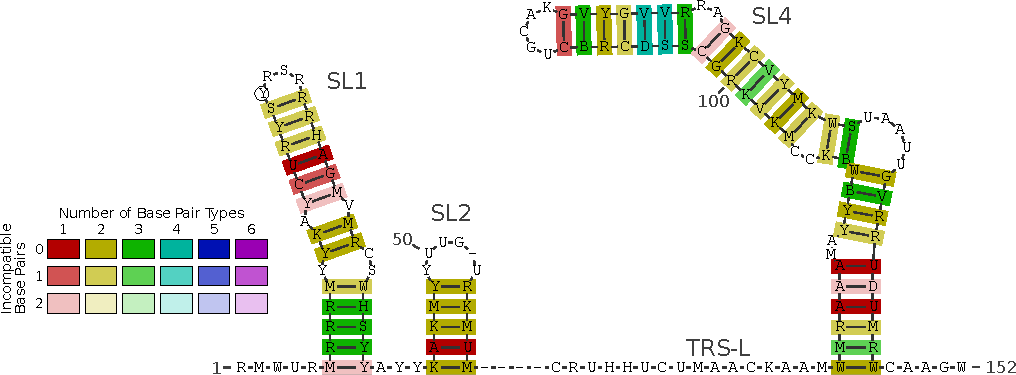
\includegraphics[width=\textwidth]{figures/color_code.pdf}
\end{frame}


\begin{frame}[c]\frametitle{Unconserved sequence, conserved structure}
	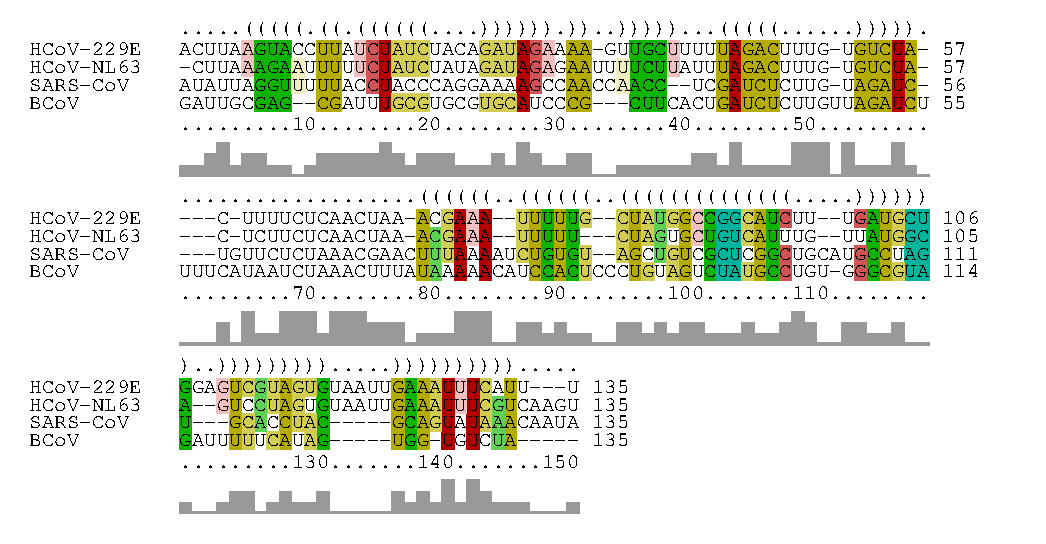
\includegraphics[width=\textwidth]{figures/cov_color_aln.ps}
\end{frame}

\begin{frame}[c]\frametitle{Compensatory Mutations in secondary structures}
	\begin{block}{Importance of such mutations}
		Compensatory mutations underline the importance of a specific secondary structure.
	\end{block}

	\uncover<2->{
	\begin{block}{But be careful!}
		If we're assuming a uniform mutation rate, every third pair of mutations is a compensatory mutation.
	\end{block}
	\small
	\begin{minipage}{0.4\textwidth}
	\centering
	\begin{tabular}{cc}
		\toprule
		A & U \\
		\midrule
		A & A \\
		A & C \\
		A & G \\
		C & A \\
		C & C \\
		\textcolor{blue}{C} & \textcolor{blue}{G} \\
		C & U \\
		\bottomrule
	\end{tabular}
	\end{minipage} \hfill \begin{minipage}{0.4\textwidth}
	\centering
	\begin{tabular}{cc}
		\toprule
		A & U \\
		\midrule
		G & A \\
		\textcolor{blue}{G} & \textcolor{blue}{C} \\
		G & G \\
		\textcolor{blue}{G} & \textcolor{blue}{U} \\
		\textcolor{blue}{U} & \textcolor{blue}{A} \\
		U & C \\
		\textcolor{blue}{U} & \textcolor{blue}{G} \\
		U & U \\
		\bottomrule
	\end{tabular}
	\end{minipage}
	}
\end{frame}

\section[LRIs]{RNA-RNA Long-Range Interactions}

\begin{frame}[c]\frametitle{Why LRIs?}
 \begin{itemize}
 	\item Interaction spans distances between a few hundred and several thousands of nucleotides
 	\item few are described in positive stranded RNA viruses
 	\item often located in loop regions (bulges, hairpins, ...)\\
 	\uncover<2->{
 	$\Rightarrow$ pseudo-knots!
 	} \uncover<3->{
 	\item LRIs may play a very important role in viral replication
 	}
 \end{itemize}
\end{frame}

\begin{frame}[c]\frametitle{How to calculate LRIs}

	\begin{minipage}[t]{0.3\textwidth}
	\begin{block}{Approach I}
	\begin{itemize}
		\item RNAduplex
		\item RNAplex
		\item RNAhybrid
	\end{itemize}
	\end{block}
	\uncover<4->{
	\begin{block}{Approach IV}
		\begin{itemize}
			\item inteRNA
			\item inRNAs
		\end{itemize}
	\end{block}
	}
	\end{minipage}
	\begin{minipage}[t]{0.3\textwidth}
	\uncover<2->{
	\begin{block}{Approach II}
	\begin{itemize}
		\item RNAcofold
	\end{itemize}
	\end{block}
	}
	\vspace*{3.5em}
	\uncover<5->{
	\begin{block}{Approach V}
		\begin{itemize}
			\item PETcofold
			\item RNAaliduplex
		\end{itemize}
	\end{block}
	}
	\end{minipage}
	\begin{minipage}[t]{0.3\textwidth}
	\uncover<3->{
	\begin{block}{Approach III}
		\begin{itemize}
			\item RNAup
			\item IntaRNA
		\end{itemize}
	\end{block}
	}
	\end{minipage}
\end{frame}

\begin{frame}[c]\frametitle{LRIscan}
	\textbf{Prediction of conserved long-range RNA-RNA interactions in full viral genomes}, 2016. M.~Fricke, M.~Marz \\
	\uncover<2->{
	$\Rightarrow$ \texttt{LRIscan}
	}
\end{frame}

\section[LRIscan]{How does LRIscan work and how do I use it?}

\begin{frame}[c]\frametitle{Workflow of LRIscan}
	\begin{center}
		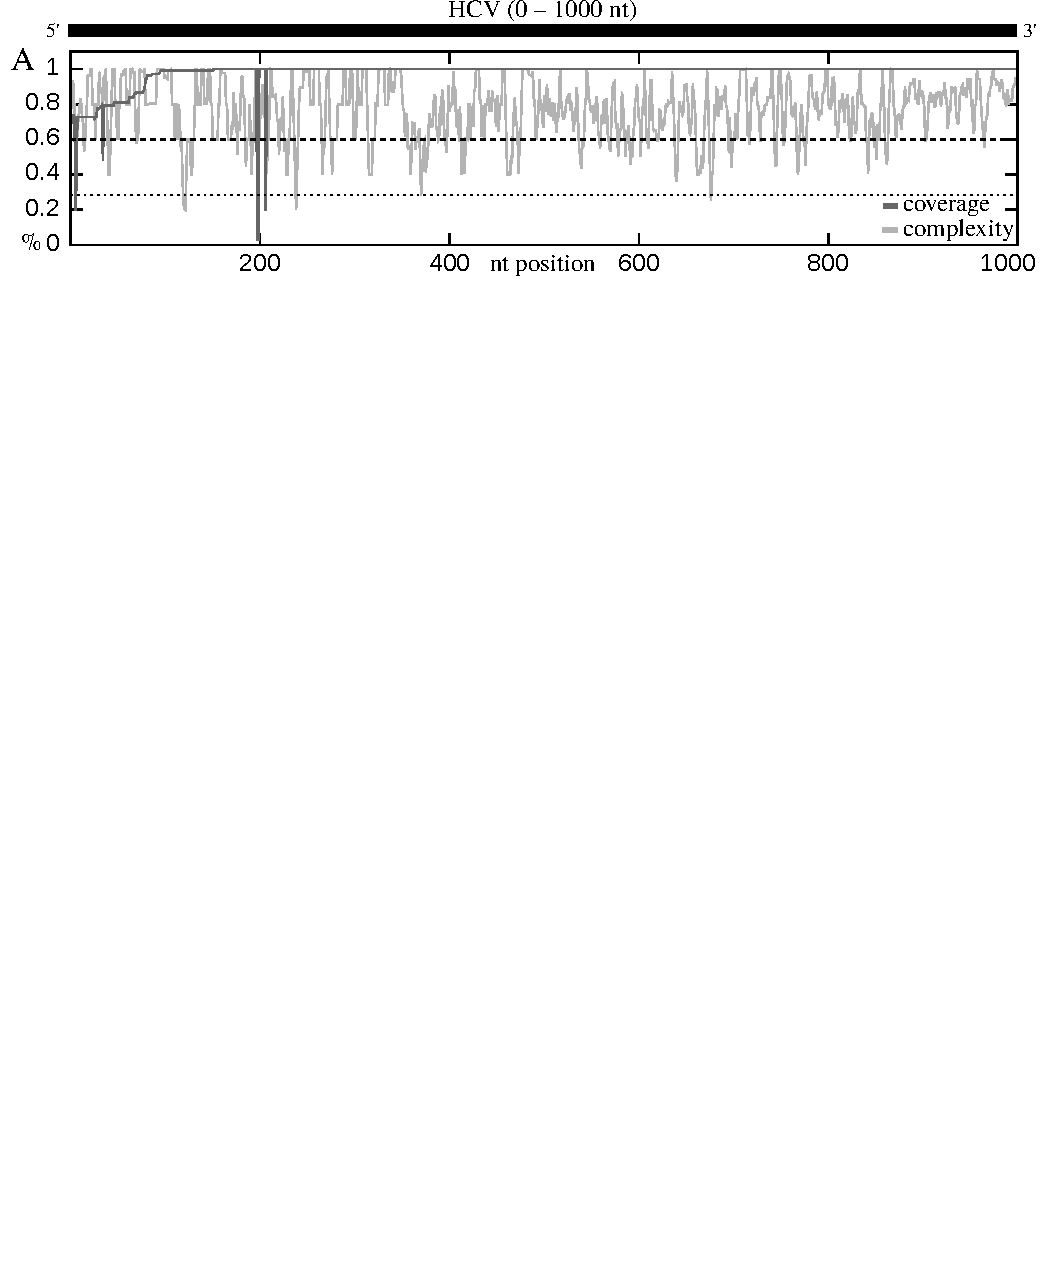
\includegraphics[height=0.9\textheight]{figures/lri_workflow_1.pdf}
	\end{center}
\end{frame}

\begin{frame}[c]\frametitle{Coverage and Complexity}
	\begin{minipage}[t]{0.45\textwidth}
		\begin{block}{Coverage of an alignment}
			Relative number of sequences that do not have a gap on a specific position.
		\end{block}
	\end{minipage} \hfill \uncover<2->{
	\begin{minipage}[t]{0.45\textwidth}
		\begin{block}{Complexity of the alignment}
			\[
				C_i = \frac{1}{m} \sum_{k=1}^{m} \frac{\lvert \delta(a_{i\dots i+s-1}^k)\rvert}{\lvert (a_{i\dots i+s-1}^k) \rvert}
			\]

			\uncover<3->{
			\[
				\delta(CCUUUGGAAA) = CUGA
			\]
			}

		\end{block}
	\end{minipage}
	}
\end{frame}

\begin{frame}[c]\frametitle{Workflow of LRIscan -- Step 2}
	\begin{center}
		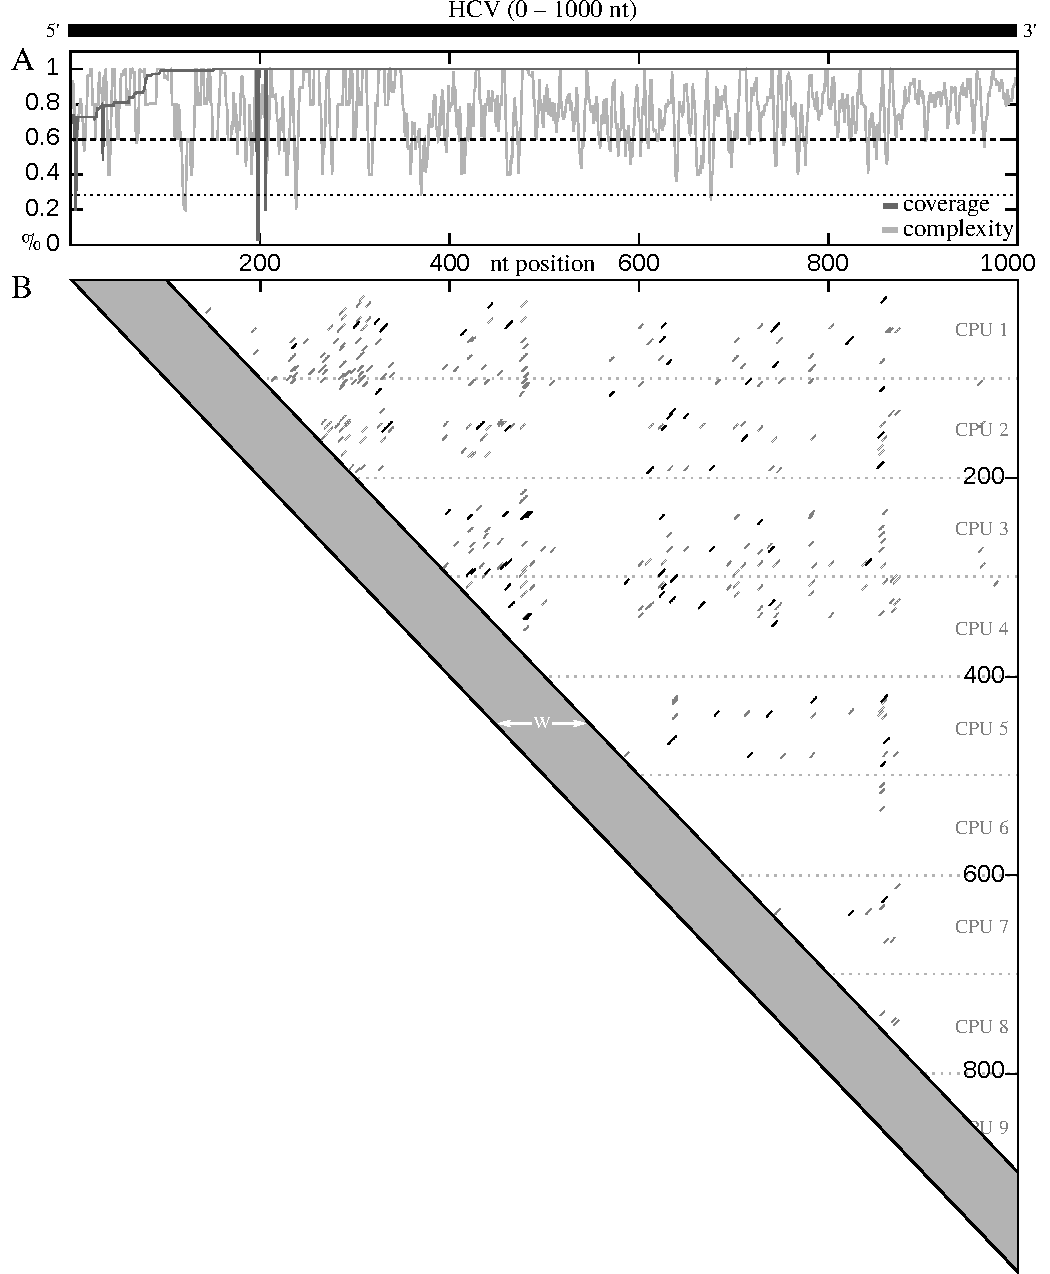
\includegraphics[height=0.9\textheight]{figures/lri_workflow_2.pdf}
	\end{center}
\end{frame}

\begin{frame}[c]\frametitle{Finding seeds}
	\[
		S_{i,j} = (S_{i-1,j+1} + 1) \cdot \Pi_{ij} \cdot \Phi_{ij}
	\]
	\begin{itemize}
		\item $\Pi_{ij}$: do at least $t$ percent of the input sequence form the basepair $(i,j)$?
		\item $\Phi_{ij}:$ do both alignment columns $A_i$ and $A_j$ meet the coverage threshold?
	\end{itemize}
\end{frame}


\begin{frame}[c]\frametitle{Workflow of LRIscan -- Step 3}
	\begin{center}
		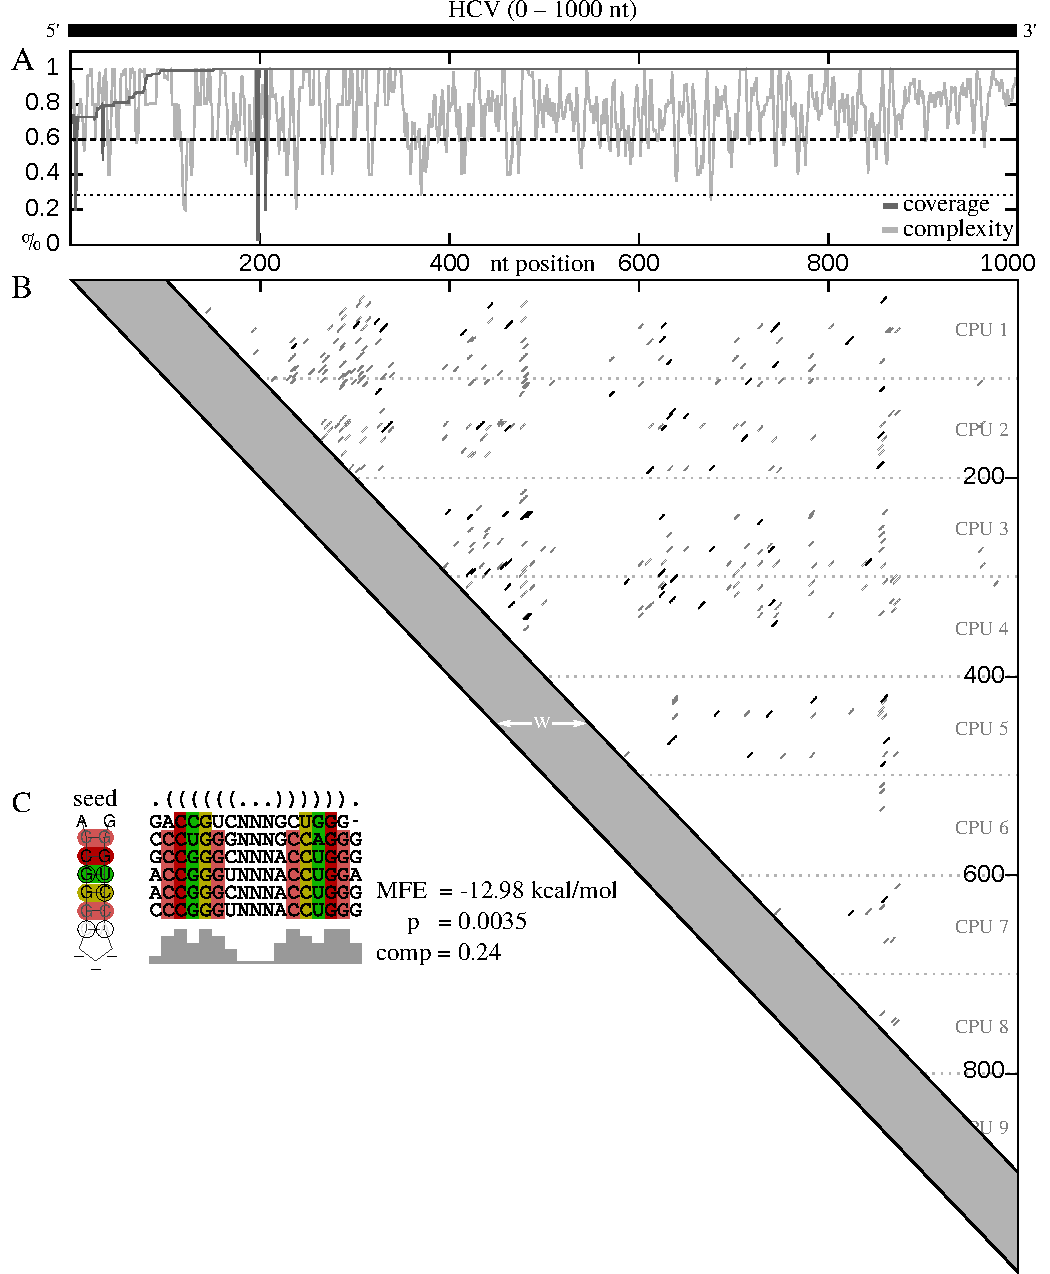
\includegraphics[height=0.9\textheight]{figures/lri_workflow_3.pdf}
	\end{center}
\end{frame}

\begin{frame}[c]\frametitle{Seed Scoring}
	\begin{itemize}
		\item z-Score analysis for each seed to measure reliability
		\item compensatory score $\tau$
	\end{itemize}
	\[
		\tau = \frac{\sum_b(u\cdot h)}{6\cdot \lvert b\rvert\cdot k}
	\]
	with:
	\begin{itemize}
		\item $u$: number of different base-pair types
		\item $h$: number of incompatible base-pairs 
	\end{itemize}
\end{frame}

\begin{frame}[c]\frametitle{Workflow of LRIscan -- Step 4}
	\begin{center}
		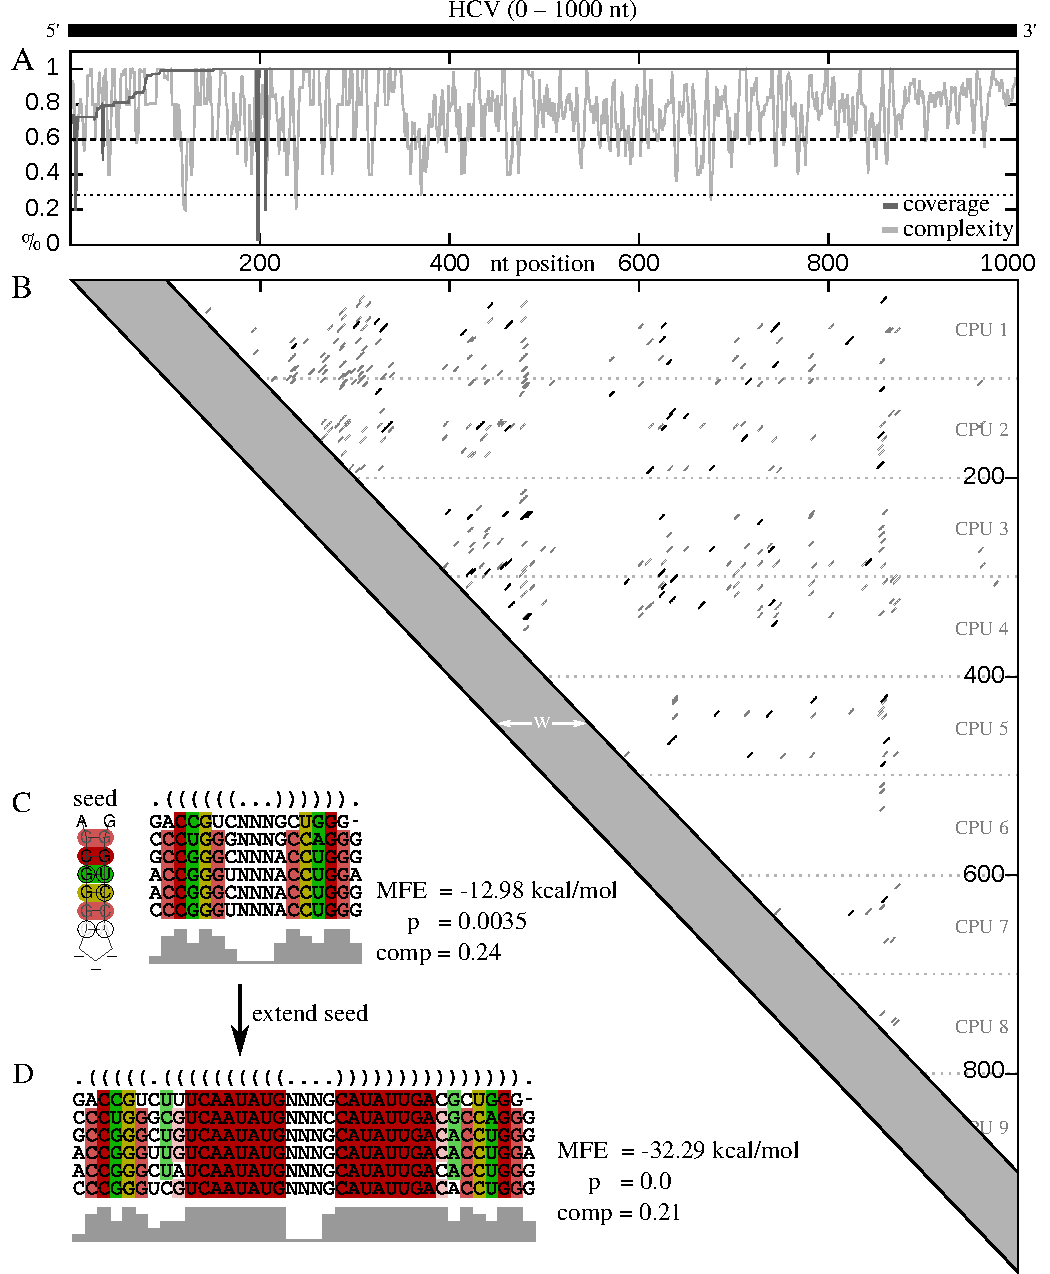
\includegraphics[height=0.9\textheight]{figures/lri_workflow_final.pdf}
	\end{center}
\end{frame}

\begin{frame}[c]\frametitle{Seed Extension}
	\begin{itemize}
		\item each seed is extended 10\,nts at the 5' (and 3' respectively)
		\item calculate MFE with RNAalifold
		\begin{itemize}
			\item hard constraints for seed region
			\item soft constraints for extension, such that intermolecular interactions are formed
		\end{itemize}
	\end{itemize}
\end{frame}

\section[Results]{LRIscan Results and Output}

\begin{frame}[c, fragile]\frametitle{LRIscan Usage}
	\begin{lstlisting}
$> ./LRIscan.rb -c 2 -f <ALIGNMENT> -o <OUTPUT>
	\end{lstlisting}

\begin{itemize}
	\item tabular output in .tsv format
	\item table and figures in .html
	\item all figures are also stored in the \texttt{ps/} directory
\end{itemize}
\end{frame}

\begin{frame}[c,fragile]{LRIscan Hands-On}
  \begin{block}{Exercise:}
    Go to \url{https://www.rna.uni-jena.de/supplements/lriscan/}\\
    \begin{enumerate}
      \item Download the MSA of the Flaviviruses
      \item Apply \texttt{LRIscan}
      \item Do not look at the results on the webpage (yet)
    \end{enumerate}
  \end{block}
  \uncover<2->{
    If you have your own dataset, roughly of the same size as the Flavivirus MSA, feel free to use it.
  }

\end{frame}

% Backup Slides. Using this macro, you'd get a slide number for each
% backup slide without increasing the maximum slide numbers of the original presentation.
% However, for this, the framenumber has to be inserted - which isn't in the template by default
\beginbackup

\begin{frame}[c]\frametitle{Coffee Break}
  \begin{figure}[htbp]
    \centering
    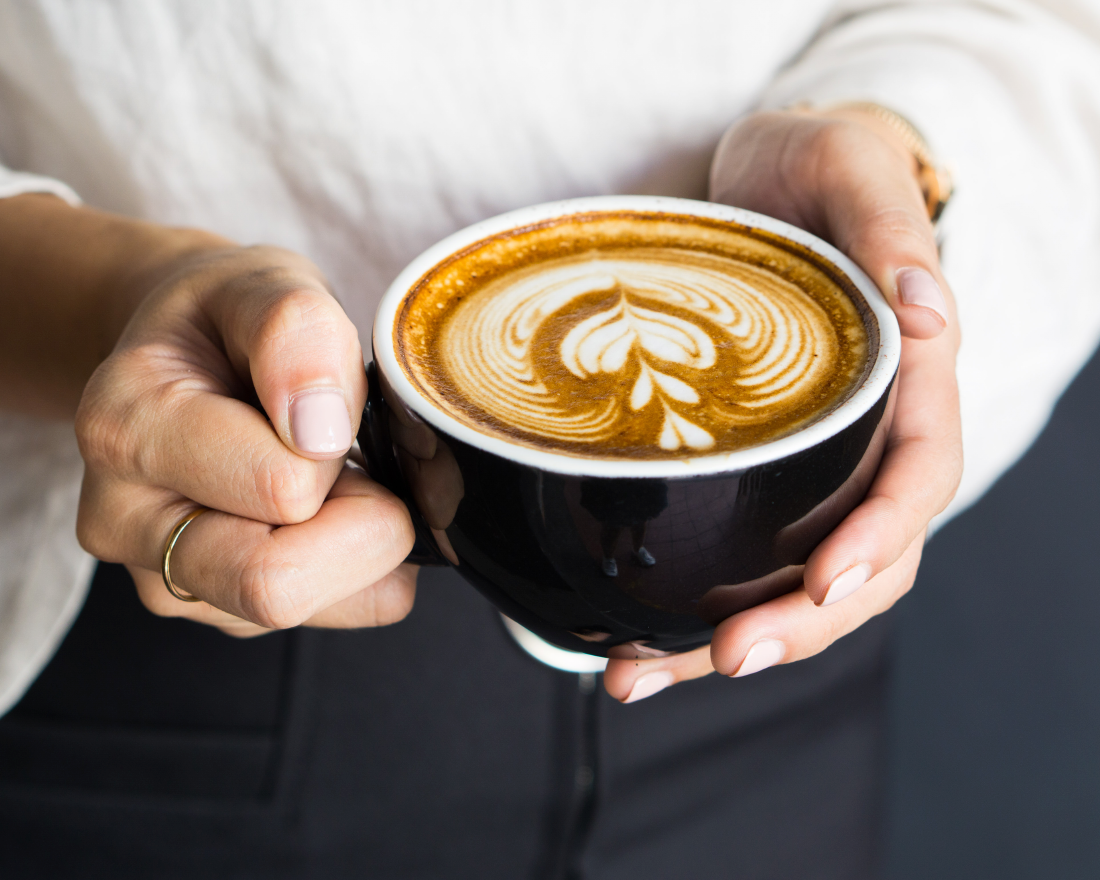
\includegraphics[width=0.65\textwidth]{coffeebreak.png}
  \end{figure}
\end{frame}

\backupend

\end{document}